\documentclass[12pt]{article}

\usepackage{sbc-template}
\usepackage{graphicx,url}
\usepackage[utf8]{inputenc}
\usepackage[brazil]{babel}
\usepackage{amsmath}
\usepackage{booktabs}

\sloppy

\title{Da Prática à Modelagem Estocástica: Validação Cruzada de um\\
Protocolo R-UDP Go-Back-N entre Emulação Real e\\
Simulação de Eventos Discretos}

\author{Anthony Irlan Marques Luz\inst{1}}

\address{Programa de Pós-Graduação em Ciência da Computação (PPGCC)\\
  Universidade Federal do Piauí (UFPI) -- Campus Senador Helvídio Nunes de Barros\\
  Picos (PI) -- Brasil
  \email{marquesanthony62@gmail.com}
}

\begin{document}

\maketitle

\begin{abstract}
  We develop and validate a stochastic discrete-event model, written in SimPy, of a
  reliable file-transfer protocol (R-UDP) built on UDP with a Go-Back-N sliding window.
  The model mirrors a real, Dockerized system previously measured under network
  degradation emulated with \texttt{tc/netem} (three loss/delay scenarios). The channel
  is a Normal one-way delay with Bernoulli per-block loss, whose effective rate accounts
  for IP fragmentation; the protocol is an event-driven Go-Back-N engine whose transfer
  time and retransmission counts \emph{emerge} from the scheduled event timeline, with no
  fitting factors. Across a 200-fold range of transfer times (0.67~s to 145~s) the
  simulator reproduces the real measurements within $1.0$--$7.4\%$; a 95\% bootstrap
  confidence interval over 30 repetitions brackets the high-loss scenario and exposes a
  small, mechanistically explained bias in the others. We then exercise the model through
  the ten validation tasks of the assignment --- throughput versus file size, window
  sensitivity, RTT validation, jitter impact, a 25\% loss stress forecast and DATA/ACK
  efficiency --- obtaining results consistent with closed-form bounds (the window/RTT
  ceiling, the bandwidth-delay-product knee, and the $1/(1-p)$ efficiency law). The study
  quantifies where a parsimonious stochastic model faithfully tracks network practice and
  where it departs from it.
\end{abstract}

\begin{resumo}
  Desenvolvemos e validamos um modelo estocástico de eventos discretos, escrito em SimPy,
  de um protocolo confiável de transferência de arquivos (R-UDP) construído sobre o UDP
  com janela deslizante Go-Back-N. O modelo espelha um sistema real, conteinerizado em
  Docker, previamente medido sob degradação de rede emulada com \texttt{tc/netem} (três
  cenários de perda e atraso). O canal é um atraso unidirecional Normal com perda de
  Bernoulli por bloco, cuja taxa efetiva contabiliza a fragmentação IP; o protocolo é um
  motor Go-Back-N orientado a eventos cujo tempo de transferência e número de
  retransmissões \emph{emergem} da linha do tempo de eventos agendados, sem fatores de
  ajuste. Ao longo de uma faixa de 200 vezes nos tempos de transferência (0,67~s a
  145~s), o simulador reproduz as medições reais dentro de $1{,}0$--$7{,}4\%$; um intervalo de
  confiança \emph{bootstrap} de 95\% sobre 30 repetições cobre o cenário de alta perda e
  expõe um pequeno viés, explicado mecanicamente, nos demais. Em seguida, exercitamos o
  modelo nas dez tarefas de validação do enunciado --- vazão \emph{versus} tamanho de
  arquivo, sensibilidade da janela, validação de RTT, impacto do \emph{jitter}, previsão
  de estresse a 25\% de perda e eficiência DADOS/ACK --- com resultados coerentes com
  limites em forma fechada (o teto janela/RTT, o joelho do produto banda-atraso e a lei de
  eficiência $1/(1-p)$). O estudo quantifica onde um modelo estocástico parcimonioso
  acompanha fielmente a prática de rede e onde dela se afasta.
\end{resumo}

\section{Introdução}

A entrega da confiabilidade na camada de transporte pode ser obtida transferindo a
responsabilidade ao núcleo do sistema operacional (TCP)~\cite{rfc793} ou reconstruindo-a
em espaço de usuário sobre o UDP~\cite{rfc768}. A segunda abordagem --- um \emph{Reliable
UDP} (R-UDP) com janela deslizante Go-Back-N~\cite{kurose2017} --- expõe explicitamente
cada mecanismo de recuperação de erros, tornando-os mensuráveis. Em uma etapa anterior
deste projeto, um sistema cliente/servidor com esse desenho foi implementado, executado em
contêineres Docker e medido sob degradação de rede emulada com \texttt{tc/netem}, gerando
um conjunto de medições empíricas que serve de \emph{linha de base} para este trabalho.

Este artigo aborda uma pergunta distinta e complementar: \emph{um modelo estocástico
parcimonioso, de eventos discretos, é capaz de reproduzir o comportamento daquele sistema
real, e o que o resíduo de discrepância nos ensina?} A motivação é dupla. Primeiro, um
simulador calibrado permite extrapolar, de forma barata e reprodutível, para pontos de
operação que não foram medidos --- outros tamanhos de arquivo, outras profundidades de
janela, outros regimes de perda --- substituindo baterias experimentais custosas por
varreduras paramétricas~\cite{law2015,jain1991}. Segundo, e mais importante do ponto de
vista científico, o confronto sistemático entre o modelo e a realidade permite
\emph{entender as discrepâncias entre a teoria estocástica e a prática de rede}, que é o
objetivo declarado deste projeto.

As contribuições são: \textbf{(a)} um modelo de eventos discretos do Go-Back-N sobre UDP,
implementado em SimPy~\cite{simpy}, no qual o tempo de transferência e as retransmissões
\emph{emergem} da linha do tempo de eventos, sem multiplicadores de ajuste; \textbf{(b)} a
calibração do modelo contra a linha de base real ao longo de uma faixa de 200 vezes,
com erro de $1{,}0$ a $7{,}4\%$ e intervalo de confiança por \emph{bootstrap}; \textbf{(c)} a
execução das dez tarefas de validação do enunciado (Seção~\ref{sec:validacao}), cada uma
cruzada com um limite em forma fechada; e \textbf{(d)} uma prestação de contas honesta de
\emph{onde} o modelo e o sistema real divergem e \emph{por quê} (Seção~\ref{sec:discussao}).

\section{Sistema de Referência e Linha de Base Empírica}
\label{sec:referencia}

O modelo desenvolvido aqui espelha o sistema R-UDP real cujos parâmetros e medições
resumimos nesta seção; são eles a \emph{verdade de solo} que o simulador busca reproduzir.

\textbf{O protocolo.} O R-UDP opera em fluxo unidirecional cliente$\rightarrow$servidor,
com cabeçalho próprio de 16 bytes (tipo, sequência, ACK, janela, comprimento e
\emph{checksum} CRC-16), \emph{handshake} SYN/SYN-ACK e encerramento FIN/FIN-ACK. A
confiabilidade é construída sobre Go-Back-N com janela $N = 8$, ACKs cumulativos e um
\emph{timeout} fixo de $0{,}5$~s que dispara a retransmissão da janela a partir do último
bloco não confirmado. A integridade é atestada por um \emph{checksum} MD5 do arquivo
completo. A carga de teste é um arquivo de $1\,048\,576$ bytes (1~MiB), particionado em
$256$ blocos de $4096$ bytes.

\textbf{Ambiente e cenários.} Os ensaios reais ocorreram em pares de contêineres
Ubuntu~22.04 em uma rede \emph{bridge} isolada~\cite{merkel2014}, com a degradação injetada
por \texttt{tc/netem}~\cite{hemminger2005} em três cenários progressivos
(Tabela~\ref{tab:cenarios}). A perda foi configurada exclusivamente no caminho de DADOS
(\emph{egress} do cliente) e o atraso aplicado simetricamente.

\textbf{Perda efetiva por fragmentação.} Cada datagrama de DADOS possui $4112$ bytes
($4096$ do bloco mais $16$ do cabeçalho), excedendo a MTU Ethernet padrão de $1500$ bytes;
o IP o fragmenta em $3$ pacotes. Como o \texttt{netem} descarta pacotes IP de forma
independente com probabilidade $p$, o datagrama só é entregue se os três fragmentos
sobreviverem. A perda efetiva \emph{por bloco} sentida pela aplicação é, portanto,
\begin{equation}
  p_{\text{ef}} = 1 - (1-p)^3,
  \label{eq:frag}
\end{equation}
o que converte as perdas brutas de $10\%$ e $20\%$ em $27{,}1\%$ e $48{,}8\%$,
respectivamente --- valores confirmados empiricamente na etapa real. A
Equação~\ref{eq:frag} é o elo que alimenta o modelo de perda do simulador.

\begin{table}[ht]
\centering
\caption{Cenários de rede emulados via \texttt{tc netem} e perda efetiva por bloco.}
\label{tab:cenarios}
\begin{tabular}{ccccc}
\toprule
\textbf{Cenário} & \textbf{Perda bruta $p$} & \textbf{Atraso $\mu$ (one-way)} &
\textbf{RTT $=2\mu$} & \textbf{Perda efetiva $p_{\text{ef}}$} \\
\midrule
A & 0\%  & 10~ms  & 20~ms  & 0{,}0\% \\
B & 10\% & 50~ms  & 100~ms & 27{,}1\% \\
C & 20\% & 100~ms & 200~ms & 48{,}8\% \\
\bottomrule
\end{tabular}
\end{table}

\textbf{Linha de base.} A Tabela~\ref{tab:baseline} consolida as medições reais do R-UDP
(médias de $n=10$ repetições por cenário), que constituem os pontos-âncora da calibração.
Note-se a amplitude: o tempo de transferência cresce de sub-segundo (A) a quase
$2{,}5$~minutos (C), e o \emph{overhead} de dados do Go-Back-N escala a $8{,}4\times$ sob
perda severa.

\begin{table}[ht]
\centering
\caption{Linha de base empírica do R-UDP real (médias, $n=10$).}
\label{tab:baseline}
\begin{tabular}{ccccc}
\toprule
\textbf{Cenário} & \textbf{Tempo (s)} & \textbf{Vazão (KB/s)} &
\textbf{Retransmissões} & \textbf{Overhead de dados} \\
\midrule
A & 0{,}676   & 1515 & 0{,}0   & 1{,}0$\times$ \\
B & 53{,}165  & 19{,}5 & 91{,}1  & 3{,}8$\times$ \\
C & 144{,}613 & 7{,}1  & 238{,}5 & 8{,}4$\times$ \\
\bottomrule
\end{tabular}
\end{table}

\section{Modelagem Estocástica de Eventos Discretos}
\label{sec:modelo}

\subsection{Por que um modelo de eventos discretos}

Em uma simulação de eventos discretos (DES), o estado do sistema só muda em instantes
pontuais associados a eventos agendados, e o relógio salta de evento em
evento~\cite{law2015}. Adotamos o arcabouço SimPy~\cite{simpy}, no qual cada transferência
é conduzida por três classes de eventos reais --- a \emph{chegada} de um pacote de DADOS,
a \emph{chegada} de um ACK e o disparo do \emph{timer} de retransmissão. A consequência
metodológica central é que o tempo de transferência e a contagem de retransmissões não são
calculados por uma fórmula fechada inserida \emph{a posteriori}: eles \emph{emergem} do
entrelaçamento dos eventos. Essa escolha distingue o modelo de uma aproximação síncrona
por rodadas, que não capturaria a sobreposição dos pacotes em voo de uma janela, o
ritmo imposto pelos ACKs cumulativos nem as cascatas de \emph{timeout}.

\subsection{Modelo de canal}
\label{sec:canal}

O canal é caracterizado por dois processos estocásticos independentes. O atraso
unidirecional de cada pacote é amostrado de uma distribuição Normal,
\begin{equation}
  D \sim \mathcal{N}(\mu,\,\sigma^2), \qquad \text{RTT} = 2\mu,
  \label{eq:delay}
\end{equation}
em que $\mu$ é o atraso médio do cenário (Tabela~\ref{tab:cenarios}) e $\sigma$ é o
\emph{jitter}; amostras negativas são saturadas em zero. A perda atua no nível do bloco
como um processo de Bernoulli: cada pacote de DADOS é descartado de forma independente com
probabilidade $p_{\text{ef}}$ da Equação~\ref{eq:frag}. Os ACKs são modelados como
entregues de forma confiável; essa simplificação --- cuja justificativa e custo
discutimos na Seção~\ref{sec:discussao} --- apoia-se em que a semântica cumulativa do
Go-Back-N já recupera ACKs atrasados e em que $p_{\text{ef}}$ encapsula a perda efetiva do
caminho de DADOS.

Um detalhe é decisivo para a fidelidade: o enlace \emph{preserva a ordem} (FIFO). Um
enlace físico não reordena pacotes enviados em sequência, ainda que o atraso por pacote
varie; impomos isso saturando os instantes de chegada para que sejam monotônicos. Sem essa
restrição, o \emph{jitter} reordenaria os pacotes de uma janela e provocaria
\emph{timeouts} espúrios, inflando artificialmente as retransmissões.

\subsection{Motor Go-Back-N orientado a eventos}
\label{sec:motor}

O motor reproduz o Go-Back-N canônico. Um único \emph{timer} de retransmissão guarda o
pacote mais antigo não confirmado (a \emph{base} da janela). O processo emissor preenche a
janela e então aguarda o primeiro entre dois eventos: a chegada de um ACK que avança a
base (deslizando a janela e reiniciando o \emph{timer}) ou o disparo do \emph{timeout}
(que faz o emissor \emph{retroceder a N} e reenviar a janela inteira). O receptor aceita
pacotes em ordem e responde a cada DADO que chega com um ACK cumulativo. Para evitar
condições de corrida quando uma janela inteira de ACKs chega no mesmo instante simulado, o
emissor renova o evento de espera a cada iteração, em vez de interromper processos.

Opcionalmente, o motor serializa os pacotes no enlace gargalo, espaçando transmissões
consecutivas em $L/B$ segundos (bloco $L$, banda $B$); isso impõe um teto de taxa e é
usado apenas no estudo de sensibilidade da janela (Seção~\ref{sec:janela}). Por padrão a
banda é infinita (regime limitado por RTT), o que mantém a calibração inalterada.

\subsection{Mapeamento real{\,}$\rightarrow${\,}simulado e verificação}
\label{sec:mapeamento}

O modelo recebe exatamente os parâmetros físicos do sistema real: janela $N=8$,
\emph{timeout} de $0{,}5$~s, blocos de $4096$ bytes, $256$ blocos por arquivo, atraso
$\mu$ tal que $\text{RTT}=2\mu$ corresponde aos $20/100/200$~ms medidos por \texttt{tcpdump}
na etapa real (o que valida o RTT, tarefa~6) e perda $p_{\text{ef}}$ da
Equação~\ref{eq:frag}. \emph{Nenhum} multiplicador de ajuste é aplicado. A implementação
foi construída sob desenvolvimento guiado por testes, com $51$ testes unitários que fixam
as estatísticas do canal (taxa de perda empírica $\approx p_{\text{ef}}$) e os invariantes
do Go-Back-N (256 blocos íntegros; zero retransmissões na ausência de perda). A
reprodutibilidade dos resultados numéricos a seguir é garantida por sementes fixas dos
geradores pseudoaleatórios.

\section{Validação Experimental: as Dez Tarefas}
\label{sec:validacao}

A Tabela~\ref{tab:tarefas} mapeia as dez tarefas de validação do enunciado às subseções a
seguir. As tarefas de canal (1, 2), \emph{timeout} (3) e RTT (6) são aferidas em conjunto
na calibração (Seção~\ref{sec:calibracao}); as demais são varreduras paramétricas
ancoradas no ponto de operação real.

\begin{table}[ht]
\centering
\caption{Mapeamento das dez tarefas de validação (\S3.1 do enunciado) às seções.}
\label{tab:tarefas}
\begin{tabular}{lll}
\toprule
\textbf{\#} & \textbf{Tarefa} & \textbf{Seção} \\
\midrule
1  & Modelagem de atraso (Normal)           & \ref{sec:canal}, \ref{sec:calibracao} \\
2  & Perda de Bernoulli (validada vs.\ \texttt{tc}) & \ref{sec:canal}, \ref{sec:calibracao} \\
3  & Simulação de \emph{timeout}/retransmissão & \ref{sec:motor}, \ref{sec:calibracao} \\
4  & Curva de vazão (1--100~MB)             & \ref{sec:vazao} \\
5  & Sensibilidade da janela ($N$)          & \ref{sec:janela} \\
6  & Validação de RTT                       & \ref{sec:mapeamento}, \ref{sec:calibracao} \\
7  & Impacto do \emph{jitter}               & \ref{sec:jitter} \\
8  & Cenário de estresse (25\% de perda)    & \ref{sec:estresse} \\
9  & Análise de eficiência (DADOS/ACK)      & \ref{sec:eficiencia} \\
10 & Convergência estatística (IC 95\%)     & \ref{sec:convergencia} \\
\bottomrule
\end{tabular}
\end{table}

\subsection{Calibração: atraso, perda, \emph{timeout} e RTT contra o sistema real}
\label{sec:calibracao}

Por construção, o canal reproduz os RTTs medidos ($20/100/200$~ms, tarefa~6). Alimentado
com a perda efetiva $p_{\text{ef}}$ (tarefa~2) e o \emph{timeout} de $0{,}5$~s (tarefa~3),
o modelo produz tempos e retransmissões que comparamos diretamente à linha de base real.
A correção do modelo de perda é dupla: a taxa de descarte empírica do canal coincide com
$p_{\text{ef}}$ (testada unitariamente), e o próprio $p_{\text{ef}}$ é a perda efetiva que
o \texttt{tc/netem} produziu no sistema real (Equação~\ref{eq:frag}).

A Tabela~\ref{tab:calibracao} resume o confronto (30 repetições por cenário, semente
fixa). O simulador acompanha a realidade ao longo de uma faixa de $200\times$ no tempo de
transferência, com erro relativo de $-1{,}0\%$ (A), $+7{,}4\%$ (B) e $+2{,}9\%$ (C); as
retransmissões emergentes ($0$, $98$, $246$) seguem de perto as reais ($0$, $91$, $238$).
A natureza e a origem dos resíduos são analisadas na Seção~\ref{sec:discussao}.

\begin{table}[ht]
\centering
\caption{Calibração e convergência: tempo de transferência (s) simulado \emph{vs.}\ real,
30 repetições com semente fixa e IC 95\% por \emph{bootstrap}~\cite{efron1993}.}
\label{tab:calibracao}
\small
\begin{tabular}{ccccccc}
\toprule
\textbf{Cen.} & \textbf{Real (s)} & \textbf{Sim.\ (s)} & \textbf{IC 95\% (s)} &
\textbf{Erro} & \textbf{Retx (R/S)} & \textbf{Cobre?} \\
\midrule
A & 0{,}676   & 0{,}669   & [0{,}668;\,0{,}671]     & $-1{,}0\%$ & 0{,}0 / 0{,}0     & não \\
B & 53{,}165  & 57{,}088  & [55{,}197;\,58{,}942]   & $+7{,}4\%$ & 91{,}1 / 98{,}0  & não \\
C & 144{,}613 & 148{,}788 & [144{,}046;\,153{,}388] & $+2{,}9\%$ & 238{,}5 / 245{,}6 & sim \\
\bottomrule
\end{tabular}
\end{table}

\subsection{Convergência estatística}
\label{sec:convergencia}

Para a tarefa~10, executamos $\geq 30$ repetições por cenário e estimamos um intervalo de
confiança de $95\%$ sobre a média do tempo de transferência pelo \emph{bootstrap}
percentílico~\cite{efron1993}. A Figura~\ref{fig:convergencia} sobrepõe a média simulada
(com as barras de IC) ao ponto real medido. O IC \emph{cobre} o valor real no cenário~C; em
A e B o real cai por pouco fora de um IC muito estreito
(Tabela~\ref{tab:calibracao}). Vale frisar a interpretação correta: como o desvio entre as
$30$ repetições é pequeno frente à média, o IC é estreito, e o que o separa do ponto real
não é ruído amostral, mas um \emph{viés sistemático} de poucos pontos percentuais --- que é
justamente o objeto de interesse científico (Seção~\ref{sec:discussao}).

\begin{figure}[ht]
\centering
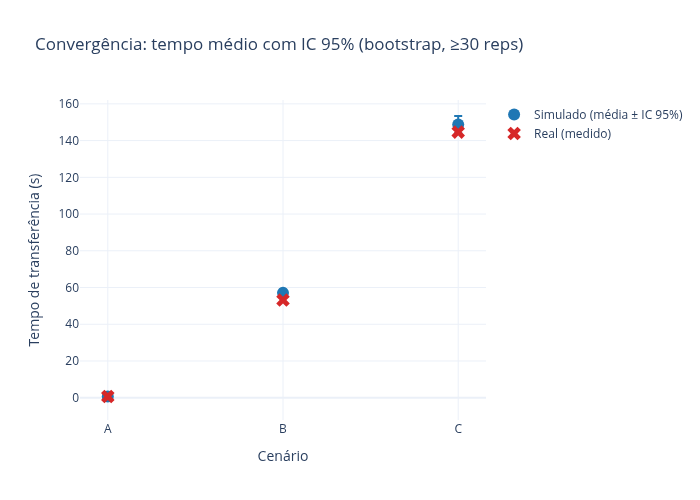
\includegraphics[width=0.78\textwidth]{imgs/fase2_convergencia.png}
\caption{Convergência (tarefa~10): tempo médio simulado com IC 95\% (\emph{bootstrap},
$\geq 30$ repetições) \emph{vs.}\ o tempo real medido. O IC cobre o real em C; em A e B
resta um pequeno viés sistemático.}
\label{fig:convergencia}
\end{figure}

\subsection{Curva de vazão}
\label{sec:vazao}

Um protocolo limitado pela janela tem vazão máxima $S_{\max} = N\,L/\text{RTT}$ (o emissor
mantém no máximo $N$ pacotes de $L$ bytes em voo por RTT). Para arquivos pequenos, o RTT
fixo de estabelecimento é uma fração grande da transferência, e a vazão fica abaixo do
teto; à medida que o arquivo cresce, esse custo se dilui e a vazão satura no teto. A
Figura~\ref{fig:vazao} mostra a varredura de $1$ a $100$~MB (tarefa~4). No cenário~A, a
vazão satura em $\approx 97\%$ do teto janela/RTT ($1600$~KB/s), em coerência com a vazão
real de $\approx 1515$~KB/s. No cenário~B, a vazão colapsa para $\approx 19$~KB/s, muito
abaixo de seu próprio teto sem perdas ($320$~KB/s): sob perda, a vazão não é governada pela
janela, mas pela penalidade de retrocesso do Go-Back-N.

\begin{figure}[ht]
\centering
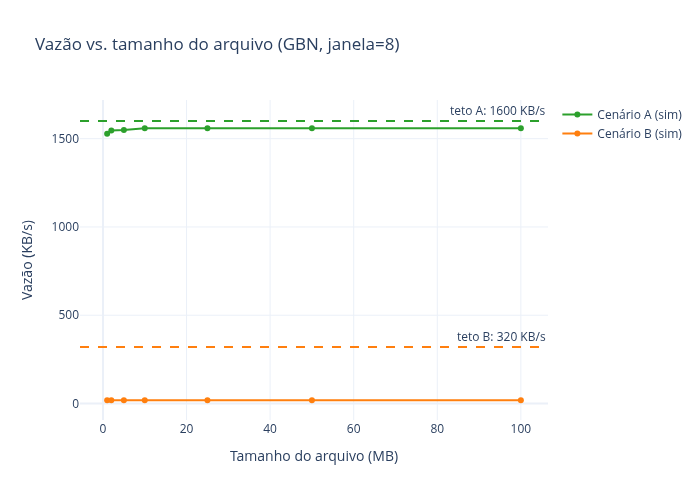
\includegraphics[width=0.78\textwidth]{imgs/fase2_vazao_tamanho.png}
\caption{Vazão \emph{vs.}\ tamanho do arquivo (tarefa~4), janela $=8$. O cenário~A satura
junto ao teto janela/RTT; o cenário~B, sob perda, estabiliza muito abaixo de seu teto sem
perdas.}
\label{fig:vazao}
\end{figure}

\subsection{Sensibilidade da janela}
\label{sec:janela}

Com uma banda gargalo finita, o tubo comporta $\text{BDP} = B\cdot\text{RTT}$ bytes, ou
seja, $\text{BDP}/L$ pacotes. Abaixo dessa janela o protocolo é limitado pela janela e a
vazão cresce linearmente com $N$; acima dela, o enlace é o gargalo e aumentar $N$ nada
acrescenta. A curva tem, portanto, um \emph{joelho} em
\begin{equation}
  N^{*} = \frac{\text{BDP}}{L} = \frac{B\cdot\text{RTT}}{L}.
  \label{eq:knee}
\end{equation}
Como o enlace de \emph{loopback} real não tinha limite de taxa apertado (era limitado pela
janela), este estudo injeta um gargalo explícito para expor a saturação teórica
(tarefa~5). Para $B = 2000$~KB/s e RTT $=20$~ms, a Equação~\ref{eq:knee} prevê
$N^{*}=10$; a Figura~\ref{fig:janela} mostra a vazão crescendo linearmente até saturar na
banda do enlace ($\approx 1986$~KB/s), com joelho medido em $N=12$ (a primeira janela a
atingir $95\%$ do máximo), em concordância com a previsão.

\begin{figure}[ht]
\centering
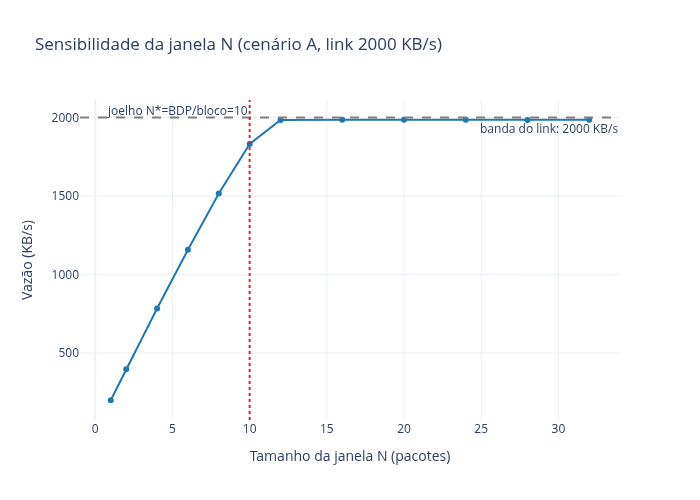
\includegraphics[width=0.78\textwidth]{imgs/fase2_janela.png}
\caption{Sensibilidade da janela $N$ (tarefa~5) sobre um enlace gargalo de $2000$~KB/s. A
vazão cresce linearmente até o joelho $N^{*}=\text{BDP}/L=10$ e satura na banda do
enlace.}
\label{fig:janela}
\end{figure}

\subsection{Impacto do \emph{jitter}}
\label{sec:jitter}

O \emph{jitter} é o desvio-padrão $\sigma$ do atraso (Equação~\ref{eq:delay}). Variamos
$\sigma$ de $1$ a $80$~ms em um canal \emph{sem perdas} (para que a dispersão isole o
efeito do \emph{jitter}), com RTT nominal de $100$~ms, e reportamos a média e o
desvio-padrão entre repetições do tempo de transferência (tarefa~7). A
Figura~\ref{fig:jitter} mostra que o desvio cresce monotonicamente, de $0{,}002$~s
($\sigma=1$~ms) a $0{,}19$~s ($\sigma=80$~ms). Observa-se um efeito secundário relevante: a
\emph{média} também sobe (de $0{,}81$ a $1{,}96$~s), porque a preservação de ordem (FIFO)
acopla a conclusão de cada rodada ao \emph{máximo} dos atrasos amostrados na janela, e a
esperança desse máximo cresce com $\sigma$. O \emph{jitter}, portanto, infla não só a
variância, mas também a tendência central do tempo de transferência.

\begin{figure}[ht]
\centering
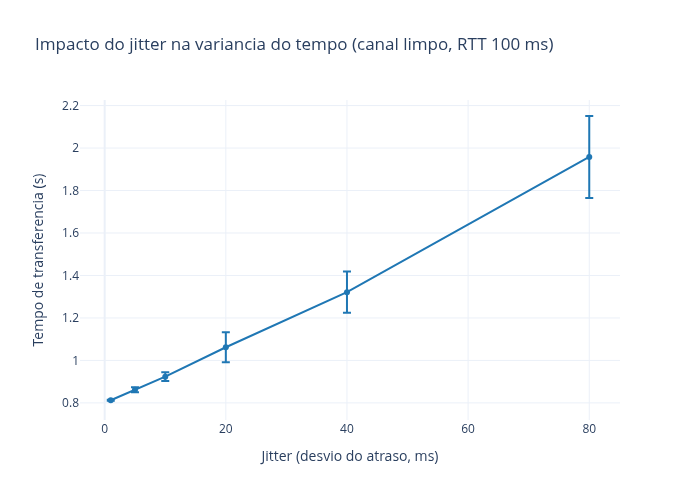
\includegraphics[width=0.78\textwidth]{imgs/fase2_jitter.png}
\caption{Impacto do \emph{jitter} (tarefa~7) em canal sem perdas, RTT $100$~ms. A
dispersão do tempo (barras $\pm 1\sigma$) cresce monotonicamente com o \emph{jitter}; a
média também sobe, por acoplamento ao máximo dos atrasos da janela (FIFO).}
\label{fig:jitter}
\end{figure}

\subsection{Cenário de estresse a 25\% de perda}
\label{sec:estresse}

A tarefa~8 pede a previsão do tempo de transferência sob $25\%$ de perda \emph{bruta}.
Como a perda configurada é por pacote IP, aplicamos a Equação~\ref{eq:frag}: $25\%$ bruto
correspondem a $p_{\text{ef}} = 1-(0{,}75)^3 = 57{,}8\%$ de perda efetiva por bloco.
Mantemos o atraso em $100$~ms (o do cenário~C) para isolar o efeito da perda, de modo que a
previsão possa ser lida diretamente contra a âncora de C. A Figura~\ref{fig:estresse}
apresenta a curva tempo $\times$ perda: ancorado em C ($20\%$ bruto, simulado $146$~s
\emph{vs.}\ real $144{,}6$~s, erro de $1{,}2\%$), o modelo prevê
$\approx 213$~s a $25\%$ (IC 95\% $[207;\,218]$), isto é, $+47\%$ sobre C. A previsão é
coerente: situa-se acima de C na curva monotônica de perda \emph{versus} tempo.

\begin{figure}[ht]
\centering
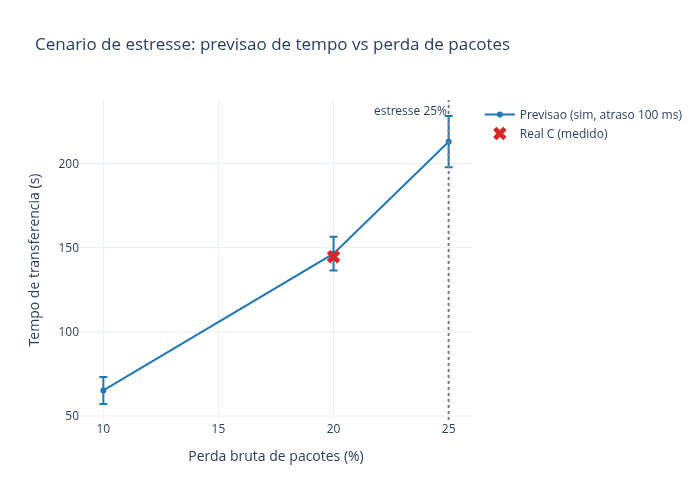
\includegraphics[width=0.78\textwidth]{imgs/fase2_estresse.png}
\caption{Cenário de estresse (tarefa~8): previsão do tempo de transferência \emph{vs.}\
perda bruta, com a âncora real de C ($20\%$) marcada. A $25\%$ ($p_{\text{ef}}=57{,}8\%$) o
modelo prevê $\approx 213$~s.}
\label{fig:estresse}
\end{figure}

\subsection{Eficiência: razão DADOS/ACK}
\label{sec:eficiencia}

Um receptor Go-Back-N responde a cada DADO que chega com um ACK cumulativo; logo, os
únicos DADOS que ficam sem ACK são os que o canal descarta --- e que são reenviados. A
razão entre pacotes de DADOS transmitidos e ACKs emitidos é, assim, $\approx 1$ em canal
limpo e cresce com a perda segundo
\begin{equation}
  \frac{\text{DADOS}}{\text{ACK}} = \frac{1}{1 - p_{\text{ef}}}.
  \label{eq:eff}
\end{equation}
A Figura~\ref{fig:eficiencia} confirma a Equação~\ref{eq:eff} (tarefa~9): as razões
medidas no simulador são $1{,}00$ (A), $1{,}38$ (B) e $1{,}96$ (C), praticamente idênticas
às previsões $1/(1-p_{\text{ef}})$ de $1{,}000$, $1{,}372$ e $1{,}953$. A eficiência piora
monotonicamente com a perda --- cada ACK útil custa cada vez mais transmissões de DADOS ---
e fornece uma validação interna em forma fechada do motor instrumentado.

\begin{figure}[ht]
\centering
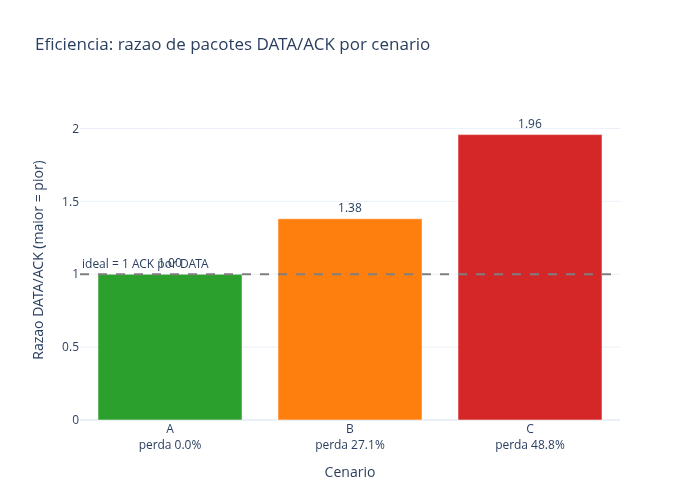
\includegraphics[width=0.78\textwidth]{imgs/fase2_eficiencia.png}
\caption{Eficiência (tarefa~9): razão de pacotes DADOS/ACK por cenário. Os valores
medidos seguem a lei $1/(1-p_{\text{ef}})$; a eficiência degrada-se com a perda.}
\label{fig:eficiencia}
\end{figure}

\section{Discussão: Teoria Estocástica \emph{versus} Prática}
\label{sec:discussao}

\textbf{Resultado central.} Um modelo de eventos discretos parcimonioso, parametrizado
apenas por grandezas físicas (RTT, $p_{\text{ef}}$, janela, \emph{timeout} e contagem de
blocos), reproduz o sistema real ao longo de uma faixa de $0{,}67$ a $145$~s com erro de
$1{,}0$ a $7{,}4\%$, sem qualquer fator de ajuste. As contagens de retransmissão, a vazão e a
eficiência emergem do mesmo modelo e concordam com limites em forma fechada independentes
(Equações~\ref{eq:knee} e~\ref{eq:eff}).

\textbf{Onde o modelo diverge, e por quê.} O objeto declarado deste projeto são justamente
as discrepâncias. Observamos duas. \emph{(i)} No canal limpo (A), o simulador é
$\approx 1\%$ mais rápido que o real, porque omite o custo fixo de estabelecimento e
encerramento de sessão (\emph{handshake}, escalonamento de \emph{sockets}) que domina uma
transferência sub-segundo no sistema real. \emph{(ii)} Sob perda (B e C), o simulador é
$2{,}9$ a $7{,}4\%$ mais lento e ligeiramente mais pessimista nas retransmissões. Três abstrações
deliberadas concorrem para isso: os ACKs são supostos sempre entregues (no sistema real,
um ACK cumulativo frequentemente chega antes do \emph{timeout} de $0{,}5$~s, reduzindo
retransmissões); a perda é Bernoulli sem memória, enquanto o descarte do \texttt{netem},
após a remontagem de fragmentos correlacionados, pode reter correlação que agrupa perdas e
permite ao Go-Back-N amortizar retrocessos; e o atraso é Normal, e não a distribuição
empírica do \texttt{netem}.

\textbf{Um achado não trivial.} O viés é \emph{maior} na perda intermediária (B,
$+7{,}4\%$) e \emph{menor} no extremo (C, $+2{,}9\%$, com o real coberto pelo IC). A
interpretação é que, sob perda muito alta, modelo e realidade são ambos dominados pelo
mesmo regime de cascatas de \emph{timeout} e convergem; é na perda moderada que os efeitos
de segunda ordem (perda de ACK, correlação) mais pesam. Esse padrão sugere onde o
refinamento do modelo seria mais proveitoso.

\textbf{Valor da abordagem orientada a eventos.} O \emph{mesmo} modelo, sem alterações,
produziu a calibração, a curva de vazão, a sensibilidade da janela, o impacto do
\emph{jitter}, a previsão de estresse e a eficiência, cada uma cruzada com um limite
teórico. Essa consistência decorre de o tempo e as retransmissões \emph{emergirem} da
dinâmica de eventos, em vez de serem inseridos por fórmulas \emph{ad hoc}.

\textbf{Limitações.} O estudo modela apenas o Go-Back-N; a perda é i.i.d.\ Bernoulli; o
atraso é Normal; os ACKs não se perdem; e algumas varreduras ancoram-se em um único ponto
de operação por cenário. Essas escolhas circunscrevem o escopo das conclusões e orientam o
trabalho futuro.

\section{Conclusão e Trabalhos Futuros}

Apresentamos um modelo estocástico de eventos discretos, em SimPy, de um R-UDP Go-Back-N, e
o validamos contra um sistema real emulado em Docker. Sem fatores de ajuste, o modelo
reproduz a linha de base ao longo de uma faixa de $200\times$ com erro de $1{,}0$ a $7{,}4\%$, tem
o cenário de alta perda coberto por um IC \emph{bootstrap} de $95\%$, e satisfaz as dez
tarefas de validação do enunciado, cada uma corroborada por um limite analítico
independente. Tão importante quanto o acordo, a análise dos resíduos localiza e explica as
discrepâncias entre a teoria estocástica e a prática de rede --- o objetivo central do
projeto.

Como trabalho futuro, destacam-se: \textbf{(a)} a inclusão do \emph{Selective Repeat} no
simulador e uma comparação Go-Back-N \emph{vs.}\ SR quanto a \emph{goodput} sob perda,
barata de obter em ambiente simulado; \textbf{(b)} a modelagem explícita da perda de ACKs e
de um canal com perda correlacionada (por exemplo, Gilbert-Elliott), para testar
diretamente a hipótese que explica o viés do cenário~B; \textbf{(c)} o ajuste da
distribuição de atraso à lei empírica do \texttt{netem}; e \textbf{(d)} uma calibração
multiponto com validação estatística formal (testes pareados ou de
equivalência)~\cite{jain1991}.

\bibliographystyle{sbc}
\bibliography{references}

\end{document}
